\documentclass[a4paper]{article}
\usepackage[top=2cm,bottom=2cm,left=2cm,right=2cm]{geometry}
\usepackage{multicol,caption}
\usepackage{lipsum}
\usepackage{graphicx}
\usepackage[parfill]{parskip}
\usepackage{authblk}
\usepackage{titlesec}
\usepackage{wrapfig}
\usepackage[utf8]{inputenc}
\usepackage{lipsum}
\usepackage{tikz}
\usepackage{chemfig}
\usepackage[version=3,arrows=pgf-filled]{mhchem}
\usepackage{enumitem}
\usepackage{siunitx}
\usepackage[ngerman]{babel}

\sloppy

%\renewcommand{\figurename}{Abbildung} % <== über babel Packet

\newbox\one
\newbox\two
\long\def\loremlines#1#2{
	\setbox\one=\vbox {
		\lipsum[#1]
	}
	\setbox\two=\vsplit\one to #2\baselineskip
	\unvbox\two}

\newenvironment{Figure}
	{\par\medskip\noindent\minipage{\linewidth}}
	{\endminipage\par\medskip}

\titlespacing*{\section}
{0pt}{1.0ex plus 1ex minus .2ex}{0.0ex plus .2ex}
\titlespacing*{\subsection}
{0pt}{1.0ex plus 1ex minus .2ex}{0.0ex plus .2ex}
\titlespacing*{\subsubsection}
{0pt}{0.5ex plus 1ex minus .2ex}{0.0ex plus .2ex}

\setlength{\parindent}{0mm}
\setlength{\parskip}{2mm}

\captionsetup[figure]{skip=1mm}

\title{NMR Spektroskopie Praktikumsbericht}
\author{Andreas Bachmann, André de Jesus Morgado, Simon de Montmollin
	\\
	ZHAW Zurich University of Applied Sciences\\
	School of Engineering
}
\date{27.05.2018}

\begin{document}
	\maketitle
	
	%Body
	\begin{multicols*}{2}
		
		\section{MAS-Rotor Testen}
			Ein Kernspinresonanz-Spektrometer besteht aus einem Magneten mit integriertem Stator (MAS), einer
			Kontrolleinheit (MAS-Controller), die Hochfrequenz-Signal generiert (Transmitter) und empfängt (Receiver/Detector),
			einem Druckgas-Kreislauf optional mit einem Wärmetauscher und einem Computer, der die Signale von der
			Kontrolleinheit aufbereitet und anzeigt (Abbildung \ref{fig:NMRSchema}).
			\begin{Figure}
				\centering
				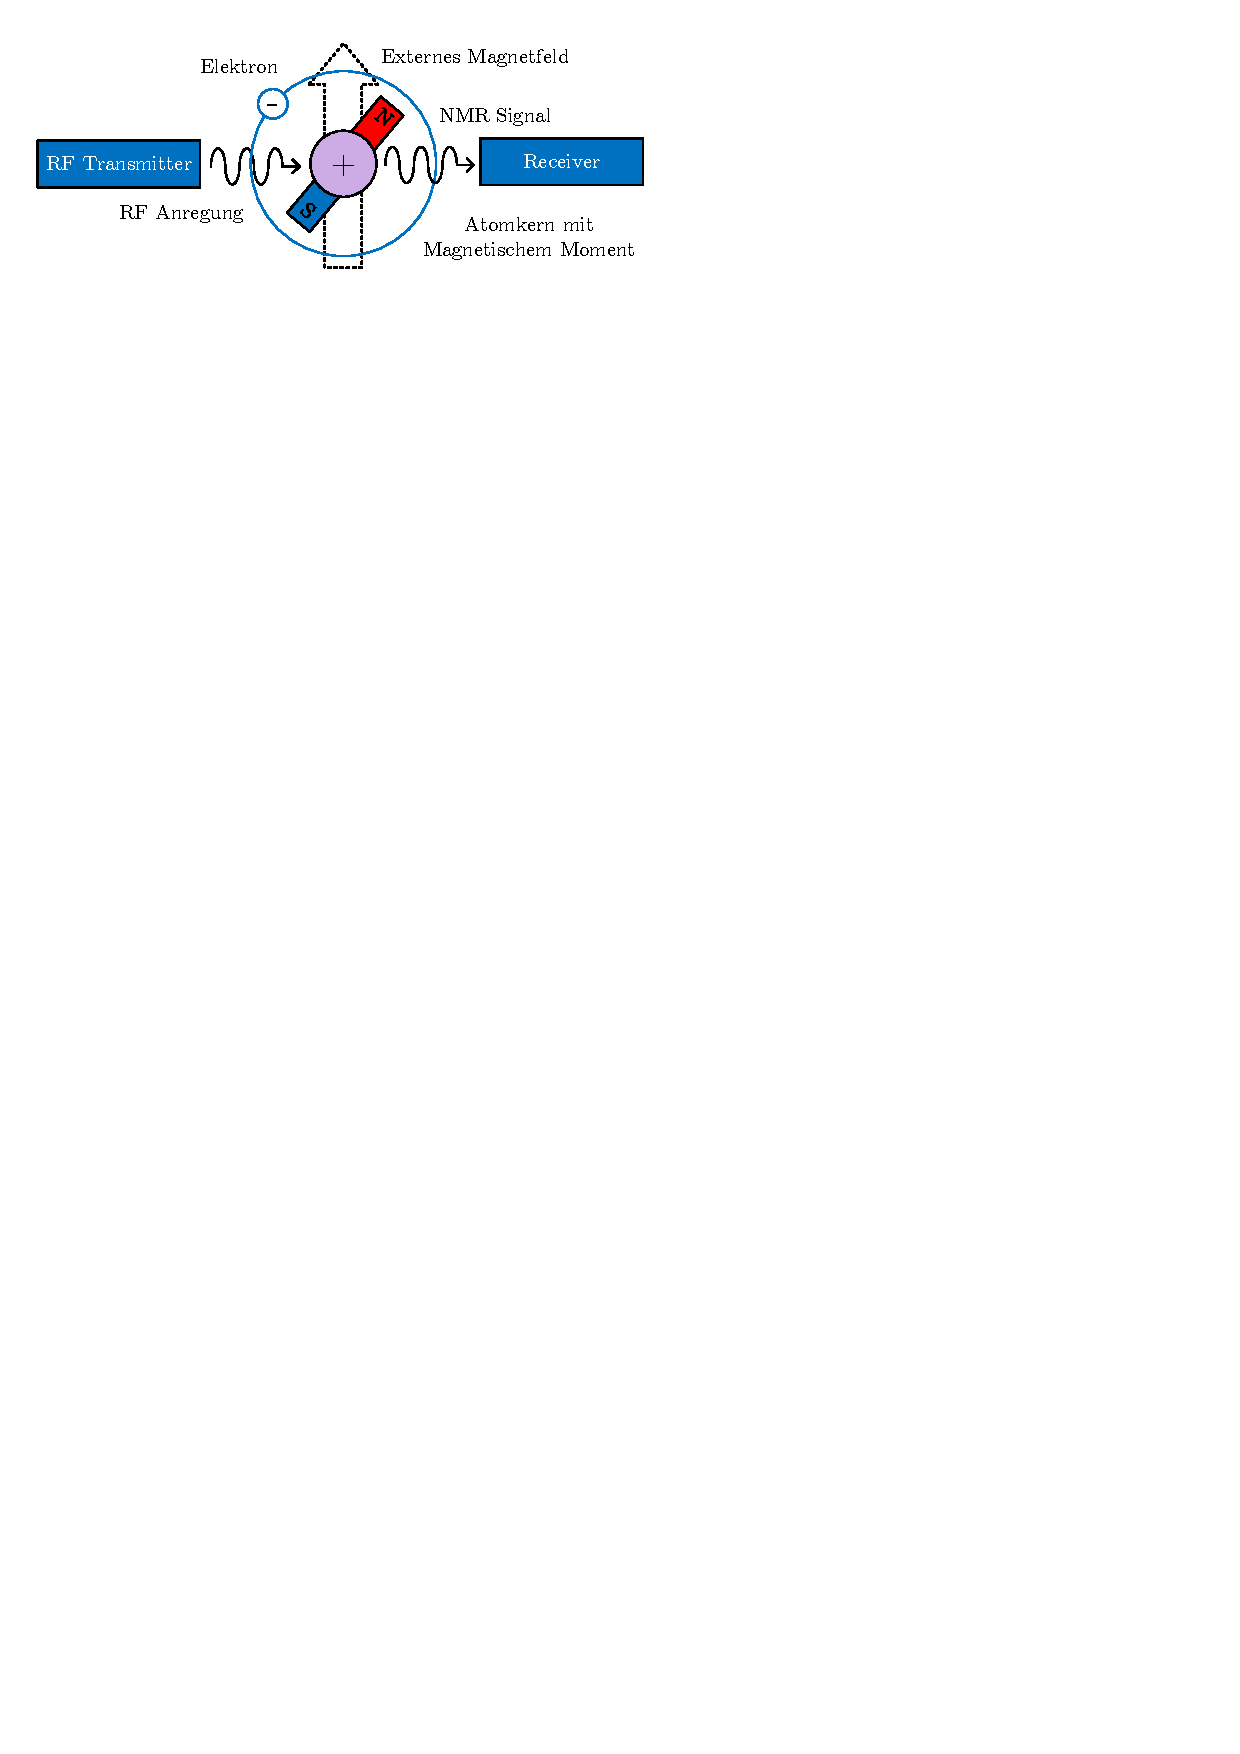
\includegraphics[trim={0.5cm 25cm 9.7cm 0.75cm},clip,width=7cm]{images/NMR_Schema.pdf}
				\captionof{figure}{Magic-Angle-Spinning (MAS) Aufbau}
				\label{fig:NMRSchema}
			\end{Figure}
		
			Dieses NMR-Spektrometer ist teuer in der Anschaffung. Zu Testzwecken wurde auf einen Magneten verzichtet.
			Die für diesen Test notwendigen Komponenten sind in Abbildung \ref{fig:device2} zu sehen.
			
			\begin{Figure}
				\centering
				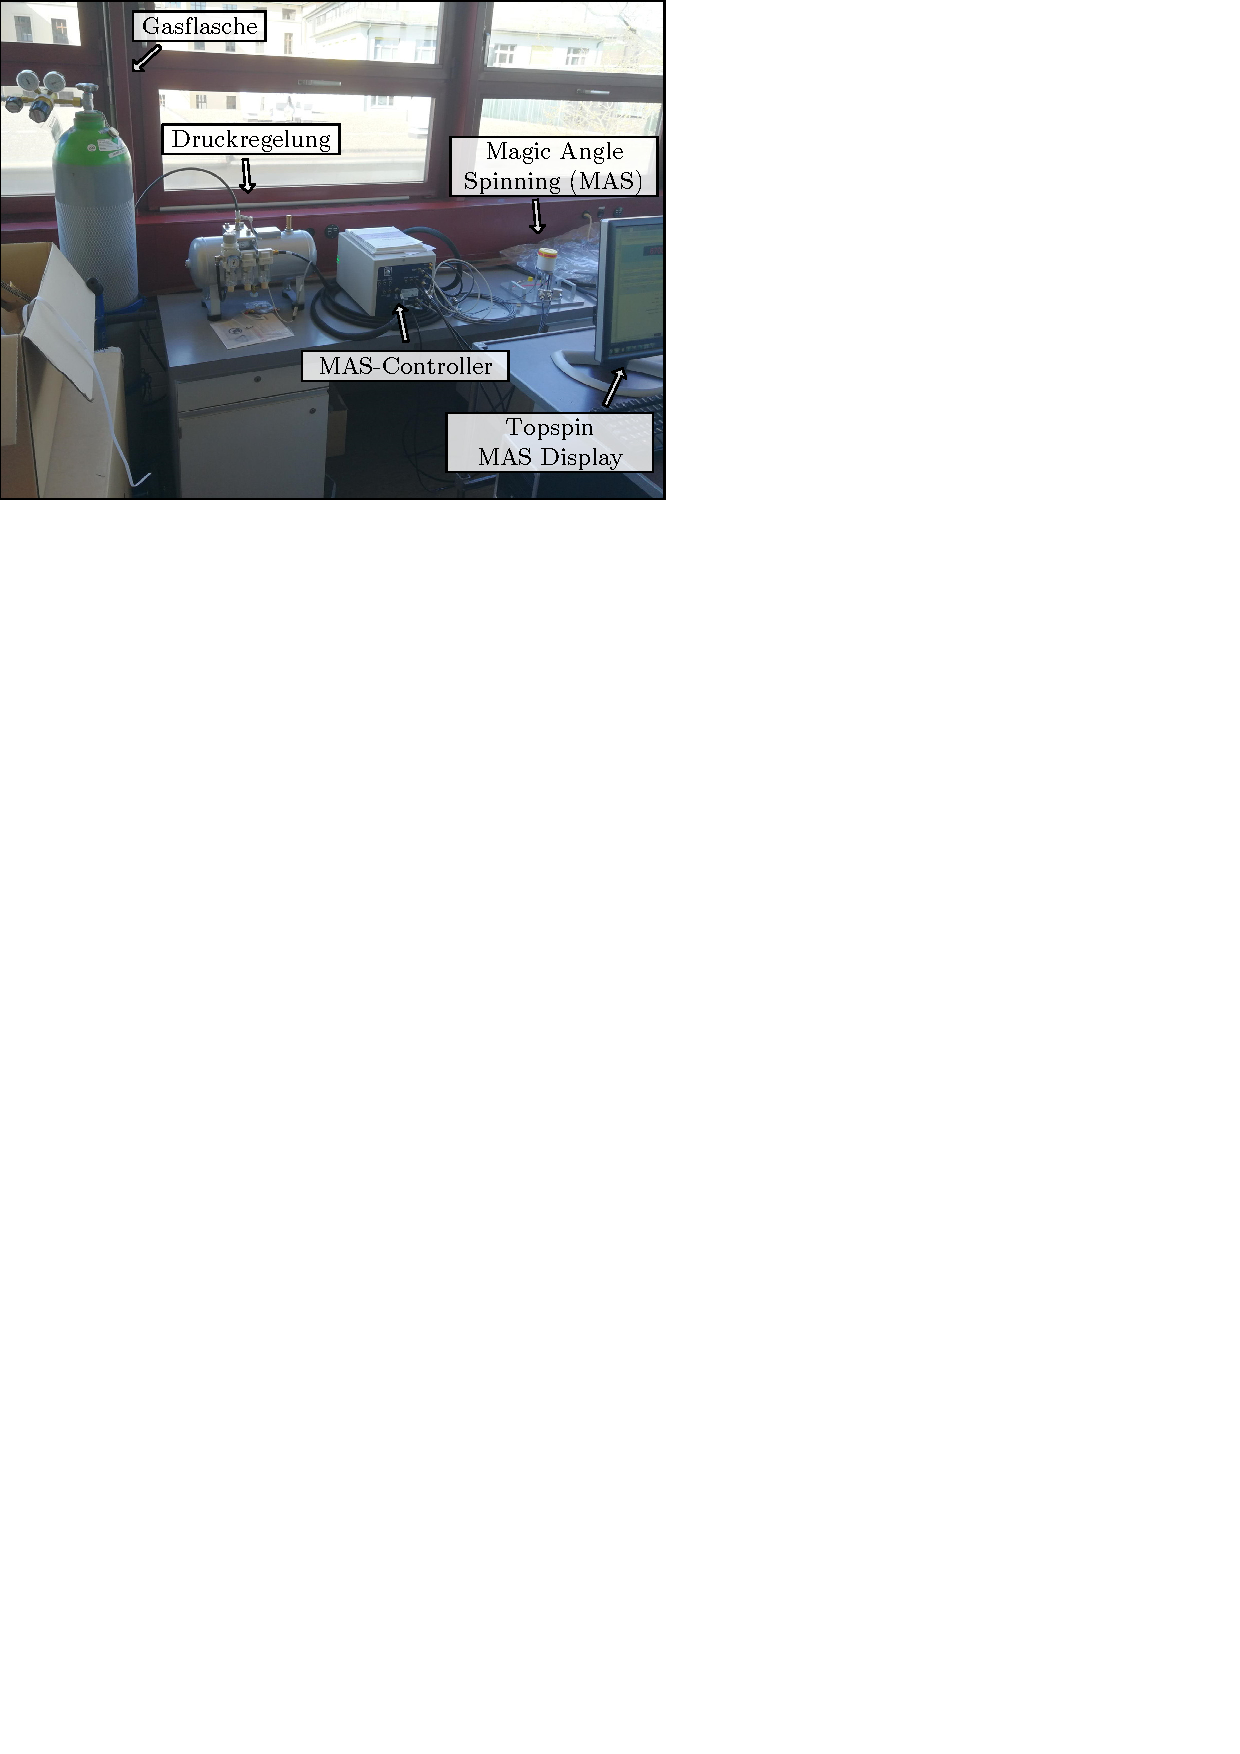
\includegraphics[trim={0cm 21.2cm 9.7cm 0},clip,width=7cm]{images/Device_2.pdf}
				\captionof{figure}{NMR Spektroskopie Geräteaufbau}
				\label{fig:device2}
			\end{Figure}
		
			\subsection{Protokoll des Rotortests}
				Mit einem Rotortest kann veranschaulicht werden, wie ein Messung einer unbekannten Substanz oder einer
				Referenzsubstanz ablaufen könnte, auch wenn kein Magnet vorhanden ist.
				
				Die Reihenfolge, wie der Test ausgeführt werden sollen, ist zu beachten. Zu beachten ist, dass
				immer eine Schutzbrille getragen werden muss.
				
				\begin{enumerate}[leftmargin=*, label=\arabic*.]
					\setlength{\itemsep}{0mm}
					\setlength{\parskip}{1mm}
					\setlength{\parindent}{0mm}
					\item Öffnen des Ventils der Gasflasche. Durch die Druckregelung wird ein konstanter Druck
					      von $\SI{8}{bar}$ gehalten.
					\item Aufschrauben der Verschlusskappe und die Versuchsprobe (Sample) in die Öffnung versenkten.
					      Die Turbine muss nach oben zur Kappe hin zeigen. Danach die Kappe wieder verschliessen.
					      Durch das Antriebsgas beginnt sich die Turbine mit dem ganzen Röhrchen (Rotor) zu Drehen.
					      Ein Rotationssensor misst die aktuelle Drehgeschwindigkeit (Abbildung~\ref{fig:device3}).
					\item In der Software kann nun die Rotationsfrequenz eingestellt werden. Der Benutzer erhöht
					      die Frequenz von $\SI{10}{kHz}$ Schritt für Schritt bis auf $\SI{67}{kHz}$. Jedes Mal
					      wenn die Soll-Frequenz (grün) erhöht wurde, regelt der MAS-Controller die Ist-Frequenz (weiss)
					      nach. Der Druck wird dabei stetig gesenkt. In der Frequenz von $\SI{67}{kHz}$ ist der Druck
					      konstant $\SI{7.1}{bar}$ (Abbildung~\ref{fig:topspin_up}).
					\item Die Analyse ist nun zu Ende und die Rotationsfrequenz wird schrittweise verkleinert. Dabei erhöht 
					      sich der Druck wieder bis der Rotor sich nicht mehr dreht. Der Enddruck hat den Wert von etwa
					      $\SI{8.6}{bar}$ erreicht. Die Druckdifferenz zwischen Maximalfrequenz und Stillstand beträgt
					      $ \Delta p = \SI{1.5}{bar}$ (Abbildung~\ref{fig:topspin_down}).
					\item Das Sample kann nun wieder vom Stator hinausgenommen und die Gasflasche geschlossen werden.
					\item Die NMR Signale vom Receiver werden in der Software noch Fourier-Transformiert und in einem
					      kontinuierlichen Spektrum angezeigt.
				\end{enumerate}
				
				\begin{Figure}
					\centering
					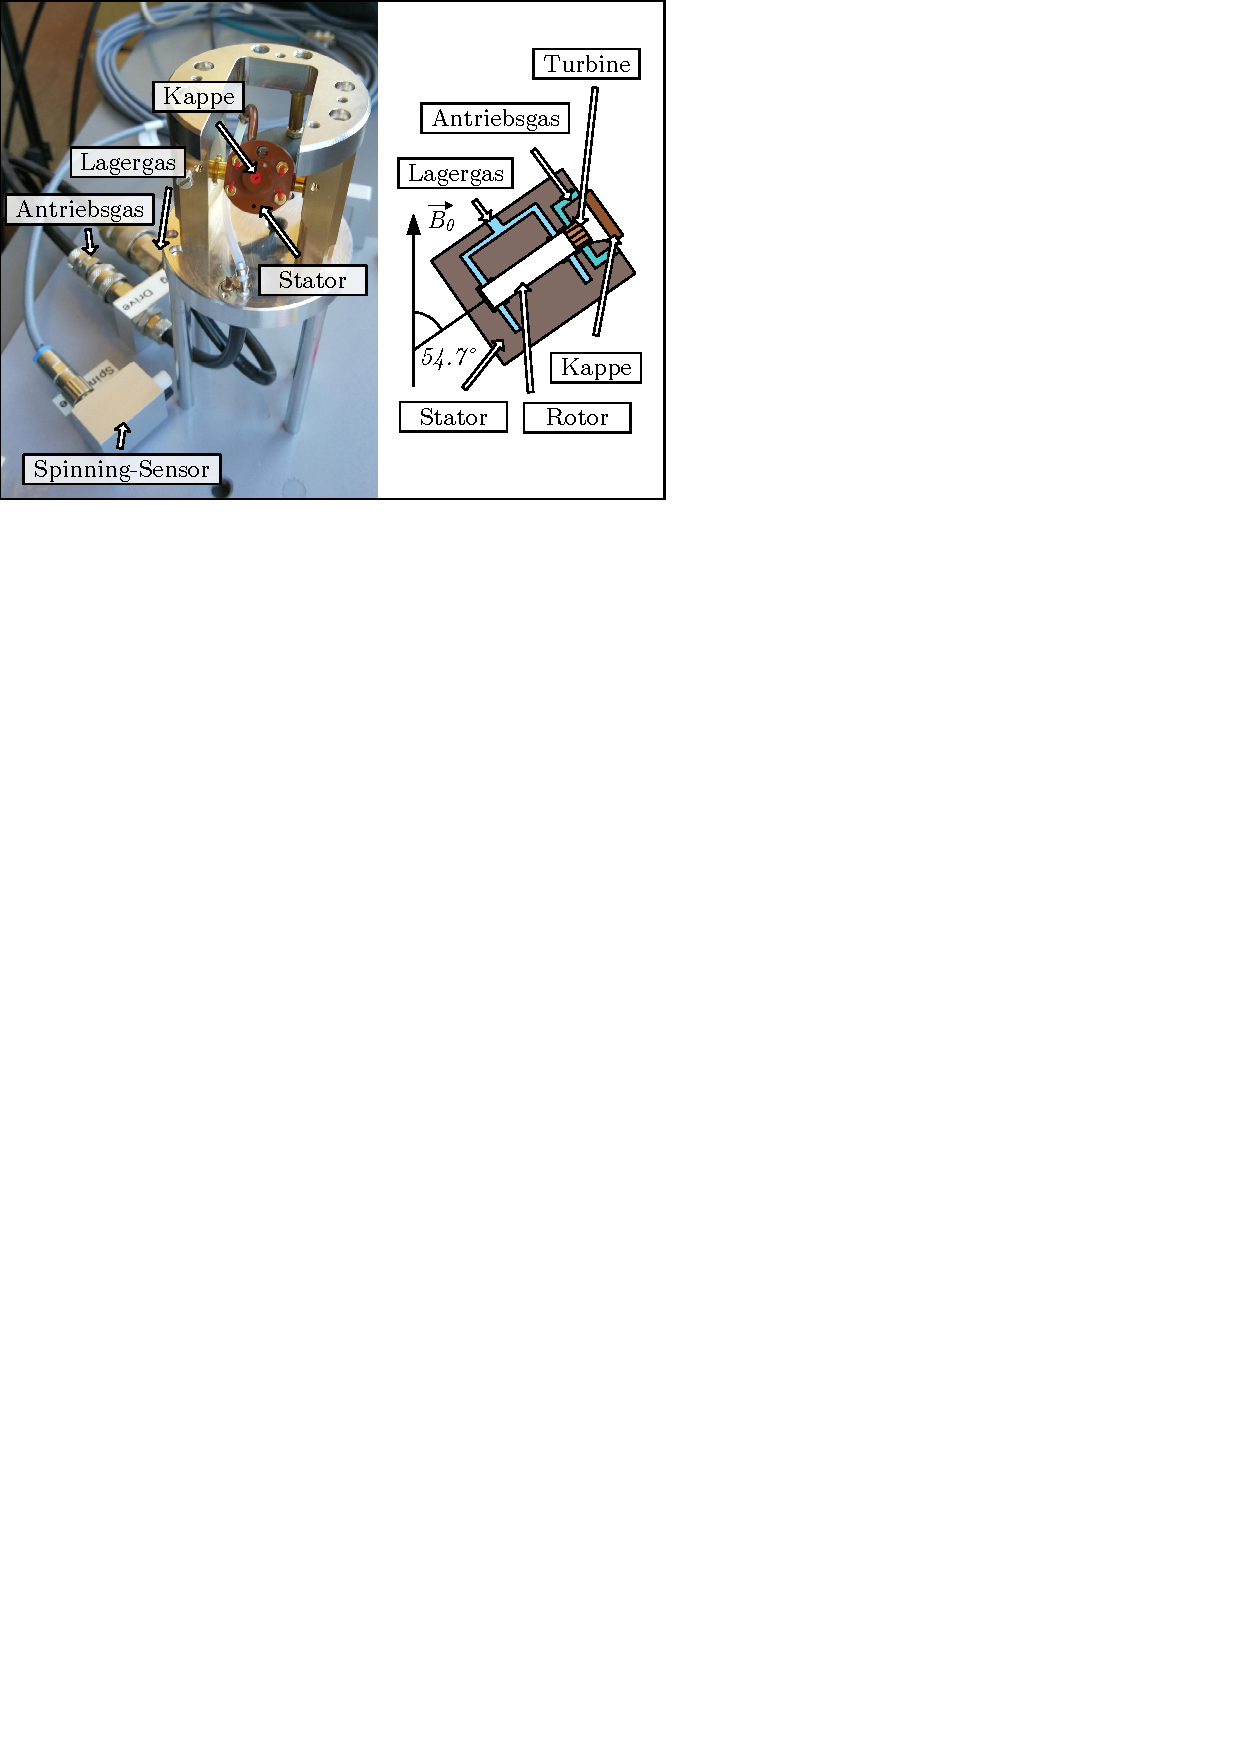
\includegraphics[trim={0cm 21.2cm 9.7cm 0},clip,width=7cm]{images/Device_3.pdf}
					\captionof{figure}{Magic-Angle-Spinning (MAS) Aufbau}
					\label{fig:device3}
				\end{Figure}
			
	\end{multicols*}


	\subsection{Resultate}
	
	\begin{Figure}
		\centering
		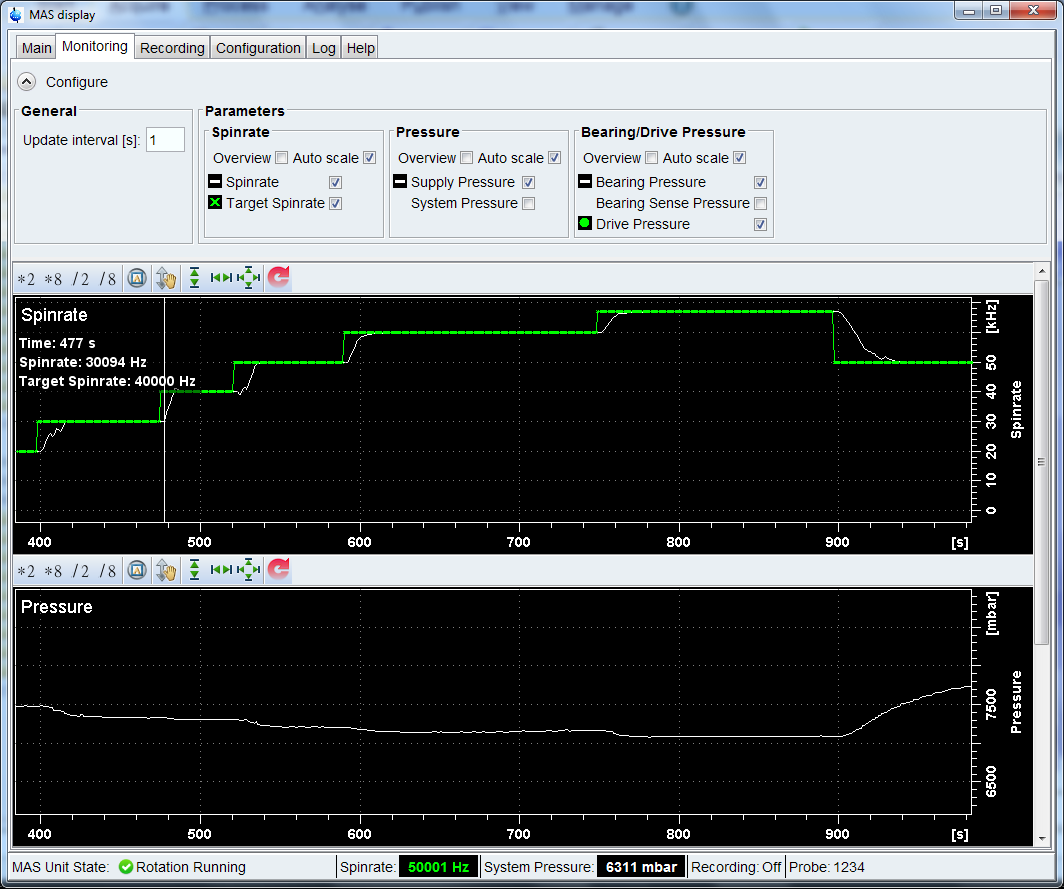
\includegraphics[width=13cm]{images/gruppe1_auf.png}
		\captionof{figure}{Erhöhen der Rotationsfrequenz}
		\label{fig:topspin_up}
	\end{Figure}
	
	\begin{Figure}
		\centering
		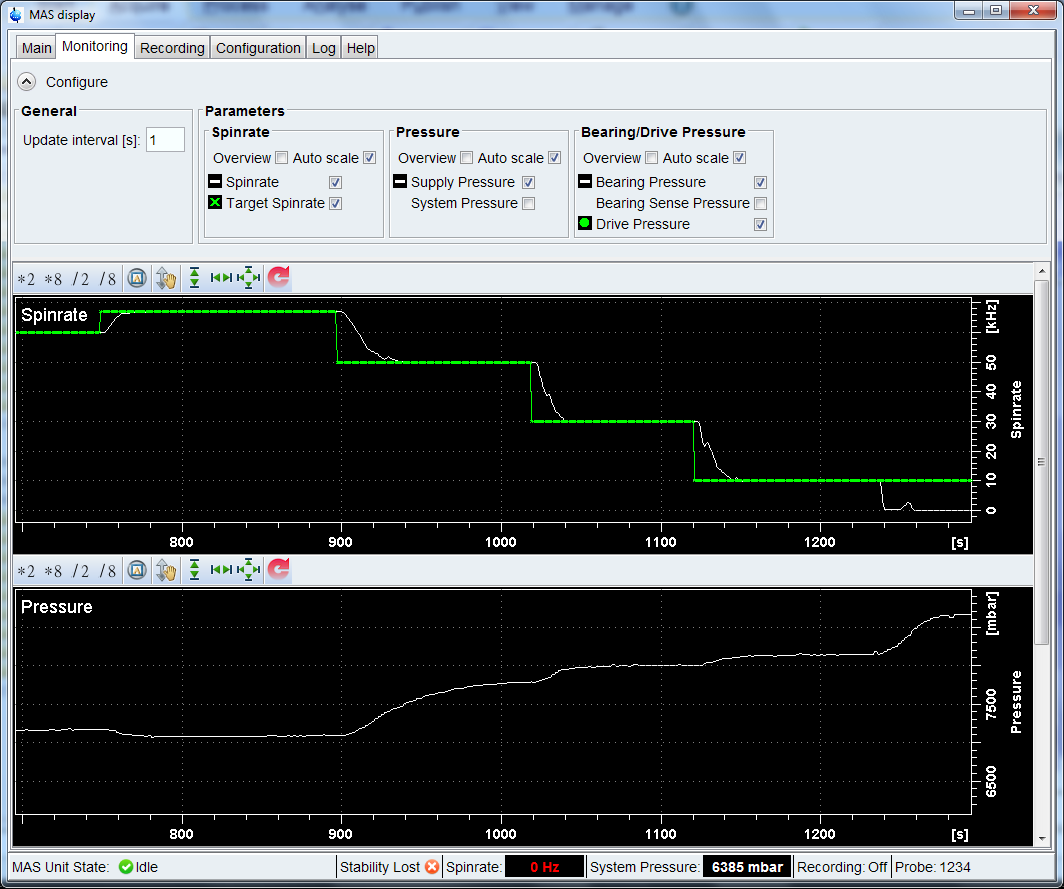
\includegraphics[width=13cm]{images/gruppe1_ab.png}
		\captionof{figure}{Erniedrigen der Rotationsfrequenz}
		\label{fig:topspin_down}
	\end{Figure}

	\pagebreak
	
	%\newgeometry{top=1cm,bottom=2cm,left=1.5cm,right=1.5cm}
	\begin{multicols}{2}
		\section{Spektrum in NMR-Software (Topspin) auswerten}
		
			\subsection{Methode}
			
			Nach der Darstellung von Enthylbenzen im Spektrogramm mit der Topspin Software, 
			kann es in drei Teile analysiert werden.
		
			\begin{Figure}
				\centering
				\begin{tikzpicture}
				\node[anchor=south west,inner sep=0] at (1cm,0cm) {
					\chemfig{C([:270]-C*6(=C(-H)-C(-H)=C(-H)-C(-H)=C(-H)-))(-[:200]H)(-[:160]H)([:45]-C([:135]-H)([:45]-H)([:315]-H))}
				};
				\node (A1) at (6cm,1cm) {\huge I};
				\node (A2) at (5.5cm,0cm) {\large Aromatischer Ring};
				\node (B1) at (0cm,5.75cm) {\huge II};
				\node (B2) at (0.5cm,4.75cm) {\large \chemfig{CH_2}};
				\node (C1) at (6cm,5.75cm) {\huge III};
				\node (C2) at (5.75cm,4.75cm) {\large \chemfig{CH_3}};
				\end{tikzpicture}
				\captionof{figure}{Valenzstrichformel von Enthylbenzen}
				\label{fig:molekul}
				\vspace*{0.5mm}
			\end{Figure}
		
			\subsection{Resultate}
				
				In Abbildung \ref{fig:spektrum_gesamt} ist das gesamte Spektrum ersichtlich.
				Die ersten Peaks bildet den aromatischen Ring ab. Der zweite das \cf{CH2}
				Molekül und der dritte und grösste, das \cf{CH3} Molekül.
				
				\begin{Figure}
					\centering
					\begin{tikzpicture}
						\node[anchor=south west,inner sep=0] at (0cm,0cm) {
							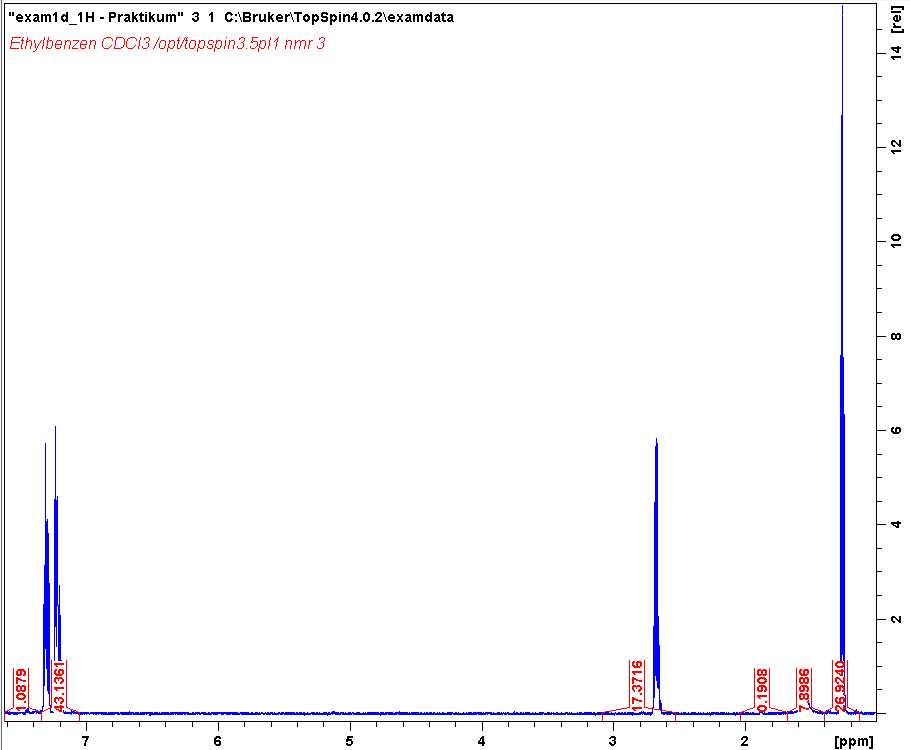
\includegraphics[width=7cm]{images/spektrum_crop.PNG}
						};
						\node (A1) at (0.4cm,3.5cm) {\huge I};
						\node[anchor=west] (A2) at (0.1cm,2.75cm) {\large Aromatischer Ring};
						\node (B1) at (5cm,3.5cm) {\huge II};
						\node (B2) at (5.1cm,2.75cm) {\large \chemfig{CH_2}};
						\node (C1) at (5.75cm,5.25cm) {\huge III};
						\node (C2) at (5.75cm,4.5cm) {\large \chemfig{CH_3}};
						\begin {scope}[red]
							\node (shift) at (2.75cm,1.7cm) {$2746$ Hz};
							\draw[<->](0.45cm,1.5cm) -- (5.05cm,1.5cm);
						\end{scope}
					\end{tikzpicture}
					\captionof{figure}{Gesamtspektrum von Ethylbenzen}
					\label{fig:spektrum_gesamt}
					\vspace*{1mm}
				\end{Figure}
			
				Der aromatische Ring in Abbildung \ref{fig:spektrum_i} zeichnet
				sich aus durch viele einzelne gleich hohe Peaks ab. Bei detaillierter Analyse haben
				diese jeweils eine Entfernung von 7.5Hz.
			
				\begin{Figure}
					\centering
					\begin{tikzpicture}
						\node[anchor=south west,inner sep=0] at (0cm,0cm) {
							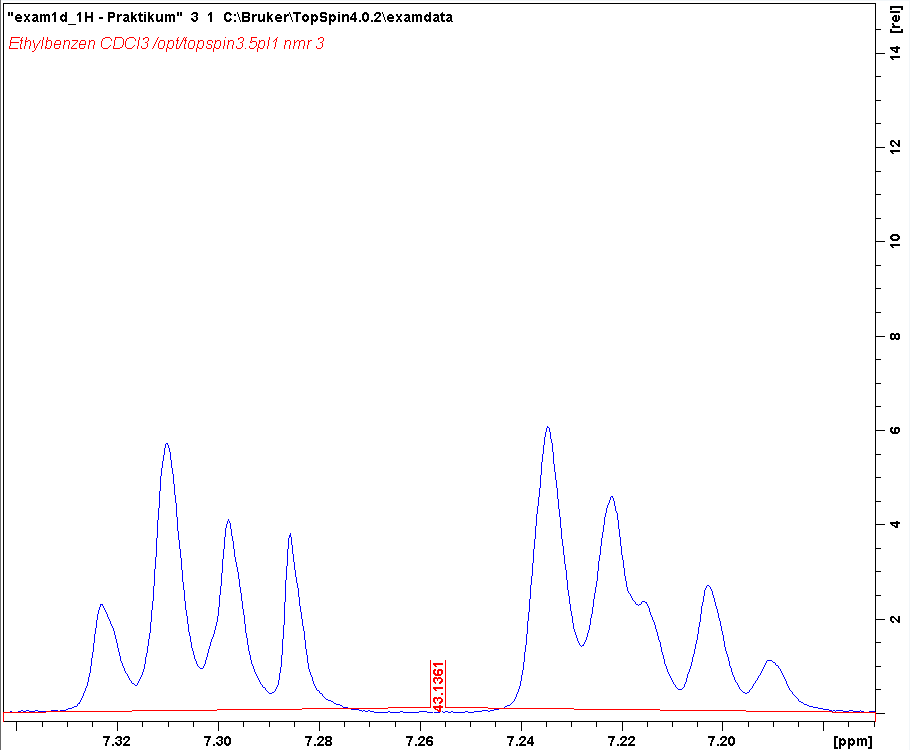
\includegraphics[width=7cm]{images/i_crop.PNG}
						};
						\node (I) at (6.3cm,5.3cm) {\huge I};
						\begin {scope}[red]
							\node (shift) at (1.5cm,3.3cm) {$7.5$ Hz};
							\draw(1.29cm,0.225cm) -- (1.29cm,3cm);
							\draw(1.76cm,0.225cm) -- (1.76cm,3cm);
							\draw[<->](1.29cm,2.7cm) -- (1.76cm,2.7cm);
						\end{scope}
					\end{tikzpicture}
					\captionof{figure}{Spektrum vom Aromatischen Ring}
					\label{fig:spektrum_i}
					\vspace*{0.5mm}
				\end{Figure}
				
				In Abbildung \ref{fig:spektrum_ii} sind weitere Peaks
				erkenntlich, jedoch weniger als bei dem aromatischen Ring. Da das \cf{CH3} Molekül die
				grösste Bindungskraft hat und somit das höchstes Spektrum, ist dieses Spektrum dem
				\cf{CH2} Molekül zuzuordnen, da es ein kleineres Spektrum aufweist.
				Auch hier ist wieder der Abstand der einzelnen Peaks auf 7.5Hz.
				
				\begin{Figure}
					\centering
					\begin{tikzpicture}
						\node[anchor=south west,inner sep=0] at (0cm,0cm) {
							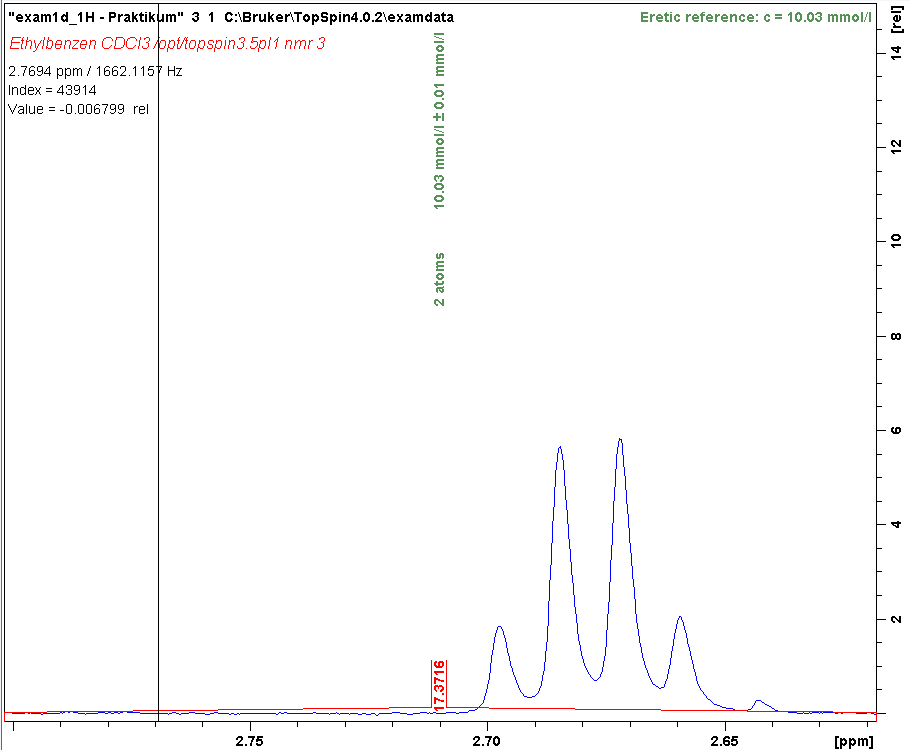
\includegraphics[width=7cm]{images/ii_crop.PNG}
						};
						\node (II) at (6.2cm,5.3cm) {\huge II};
						\begin {scope}[red]
							\node (shift) at (4.5cm,3.3cm) {$7.5$ Hz};
							\draw(4.32cm,0.225cm) -- (4.32cm,3cm);
							\draw(4.77cm,0.225cm) -- (4.77cm,3cm);
							\draw[<->](4.32cm,2.7cm) -- (4.77cm,2.7cm);
						\end{scope}
					\end{tikzpicture}
					\captionof{figure}{Spektrum von \cf{CH2}}
					\label{fig:spektrum_ii}
					\vspace*{0.5mm}
				\end{Figure}
				
				In der letzten Abbildung \ref{fig:spektrum_iii} sind weniger Peaks zu sehen, jedoch höhere.
				Daraus folgt, dass dieses Spektrum dem \cf{CH3} Molekül zugeordnet wird, aufgrund der starken
				Bindungskraft.
				
				\begin{Figure}
					\centering
					\begin{tikzpicture}
						\node[anchor=south west,inner sep=0] at (0cm,0cm) {
							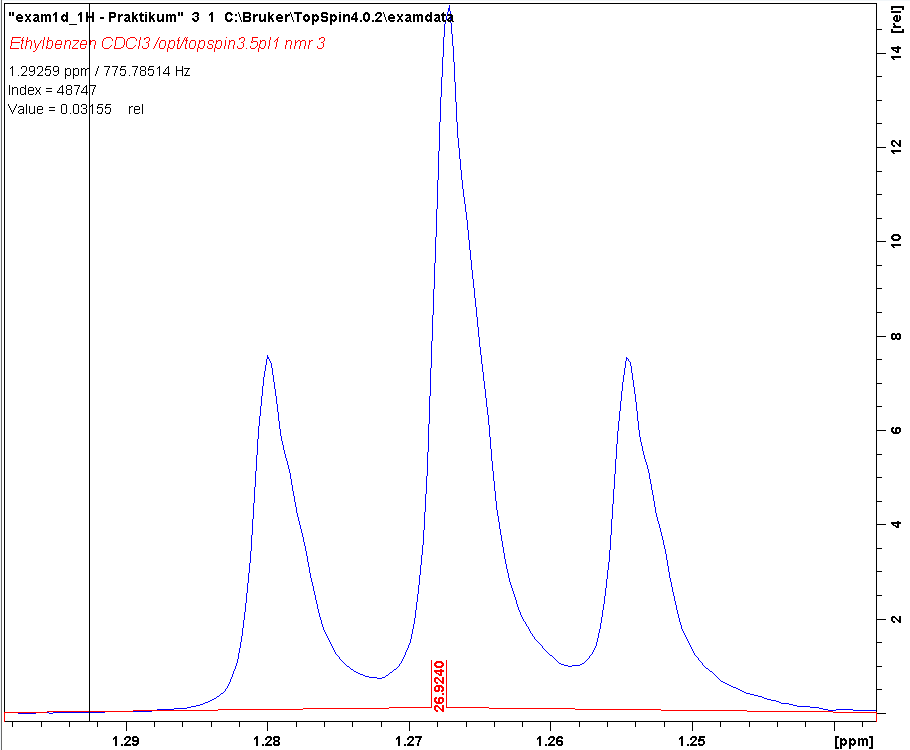
\includegraphics[width=7cm]{images/iii_crop.PNG}
						};
						\node (III) at (6.1cm,5.3cm) {\huge III};
						\begin {scope}[red]
							\node (shift) at (4.2cm,3.6cm) {$7.6$ Hz};
							\draw(3.46cm,0.225cm) -- (3.46cm,5.6cm);
							\draw(4.84cm,0.225cm) -- (4.84cm,3.5cm);
							\draw[<->](3.46cm,3.3cm) -- (4.84cm,3.3cm);
						\end{scope}
					\end{tikzpicture}
					\captionof{figure}{Spektrum von \cf{CH3}}
					\label{fig:spektrum_iii}
					\vspace*{0.5mm}
				\end{Figure}
	\end{multicols}
\end{document}